\part{Билеты на отл}
\setcounter{section}{0}

\section{Описание пифагоровых троек, используя гауссовы числа.}
\Def Пифагорова тройка: $(a, b, c): a, b, c \in \N; a^2 + b^2 = c^2$

\Note Можно рассматривать только взаимно простые числа: если любые два числа из тройки имеют общий множитель, то и третье число делится на него.

\Th 
Если $a^2 + b^2 = c^2$ для попарно взаимно простых чисел $a, b$, то с точностью до перестановки a и b и их знака найдутся такие целые числа $m, n$, что $a = m^2 - n^2, b = 2mn, c = m^2 + n^2$

\Proof

1. Перепишем исходное равенство следующим образом: $a^2 + b^2 = (a+bi)(a-bi) = c^2$. 

2. $a+bi$ и $a - bi$ взаимно просты: $(a+bi, a-bi) = (a+bi, 2a)$. Заметим, что $(a + bi, 2) = 1$, т.к. иначе $c^2$ кратно 2, а значит, и 4, а значит, и a, и b, кратны 2 (т.к. иначе $c^2$ либо нечётное, либо кратно 2, но не кратно 4), а это противоречит взаимной простоте $a, b, c$. Тогда $(a+bi, a-bi) = (a+bi, 2a) = (a+bi, a) = (bi, a) = (a, b) = 1$ в силу взаимной простоты.

3. Произведение $a+bi$ и $a - bi$ - квадрат какого-то числа, получается, всякое простое число, которое встречается в разложении $c^2$ (а оно встречается чётное число раз), встречается и в разложении либо $a + bi$, либо $a-bi$ то же число раз. Таким образом, $a + bi = u(m + ni)^2$, где $u$ - обратимый элемент. Сделав замену при необходимости, можно избавиться от u; Таким образом, $a + bi = (m + ni)^2$.

4. Тогда $a = m^2 - n^2, b = 2mn$; $a - bi = \overline{a + bi} = \overline{(m + ni)^2} = (\overline{m + ni})^2 = (m - ni)^2$; тогда $c = (m + ni)(m - ni) = m^2 + n^2$ с точностью до знака.
\EndProof

\section{Теорема Ферма при $n = 3$ (формулировка). Описание свойств элемента $\lambda = 1 - \omega \in Z[\omega]$: сравнимость по модулю $\lambda$, $\lambda^2$, $\lambda^4$. Если $\lambda$ делит $x^3 + y^3$ для взаимно-простых $x, y$, то $(x + y, x + \omega y) = (x + y, x + \omega^2 y) = (x + \omega^2y, x + \omega y) = \lambda$}
\Th (Великая теорема Ферма при $n = 3$)
	Уравнение $x^3 + y^3 = z^3$ не имеет нетривиальных целочисленных решений.
\\
\\
В следующих трех билетах мы будем доказывать теорему Ферма. 
\\
Сразу сделаем несколько замечаний. Прежде всего, удобнее
говорить о нетривиальных решениях в целых числах (то есть о таких, в которых ни одно число не равно нулю). Тогда можно
говорить как об уравнении $x^3 + y^3 = z^3$, так и об уравнении $x^3 + y^3 + z^3 = 0$ Из последнего следует, что переменные можно менять местами друг с другом. \\
Давайте сначала найдём идею доказательства, а потом его строго запишем.
\\
Мы хотим использовать числа Эйзенштейна для доказательство этого факта. Почему? Дело в том, что в числах Эйзенштейна есть кубический корень из 1. Поэтому мы можем разложить $x^3 + y^3$ на линейные сомножители. А именно, $x^3 + y^3 = (x + y)(x + \omega y)(x + \omega^2y)$  (это равенство можно проверить непосредственно). \\
Итак, мы будем доказывать, что уравнение
$x^3 + y^3 = z^3$ не
имеет нетривиальных решений в числах Эйзенштейна. Как и в пифагоровых тройках, можно предполагать попарную взаимную
простоту x, y, z. Мы имеем равенство:
\begin{center}
    $(x + y)(x + \omega y)(x + \omega^2y) = z^3$
\end{center}
Если продолжать аналогию с пифагоровыми тройками, надо выяснить взаимную простоту трёх сомножителей. Заметим, что
$(x + y, x + \omega y) = ((1 - \omega)y, x + y)$.
Что за число $1 − \omega$? Его норма, как легко посчитать, равна 3,
значит, это простое число Эйзенштейна. Для сокращения записи обозначим
$\lambda = 1 - \omega$. Вернёмся к наибольшему общему делителю $x + y$ и $x + \omega y $.
\\
\\
\Lemma
 Если $\lambda$ делит $x^3 + y^3$ для взаимно-простых $x, y$, то $(x + y, x + \omega y) = (x + y, x + \omega^2 y) = (x + \omega^2y, x + \omega y) = \lambda$
 \\
 \Proof
Так как y и x + y не имеют общих делителей, то
$(x + y, x + \omega y) = (\lambda y, x + y) = (\lambda, x + y) = \lambda$ или 1.
\\
Далее $(x + y, x + \omega^2 y) = (x + y,(1 - \omega^2)y) = (x + y, \lambda y) = (x + y, x + \omega y)$,
\\
$(x + \omega y, x + \omega^2y) = (x + \omega y, \lambda \omega y) = (x + \omega y, \lambda y) = (x + y, x + \omega y)$.
То есть либо все три сомножителя попарно взаимно просты, либо у каждой пары наибольший общий делитель равен $\lambda$. Первый случай невозможен, так как по условию $\lambda$ делит $x^3 + y^3$
\EndProof
\\
\\
\Lemma
	$z \in \Z[\omega]$ либо делится на
    $\lambda$, либо сравним с обратимым элементом по модулю 3. Более того, если $\lambda \nmid z$. Тогда $z^3 \equiv_9 \pm 1$.

\Proof
Пусть x = $a+b\omega$. По модулю 3 можно представить x как $a_0+b_0\omega$, где $a_0, b_0$ $\in$ $\{0, −1, 1\}$. Из 9 вариантов 6 задают
обратимый элемент, а оставшиеся 3 - это $0, 1 -\omega = \lambda, -1 + \omega$ =
$-\lambda$, то есть делятся на $\lambda$. 
\\
\\
С другой стороны, пусть $x = 3w + u$, где u — обратимый элемент. Тогда
$(3w + u)^3 = 27w^3 + 27w^2u + 9wu^2 + u^3  \equiv_3 u^3  \equiv_9 \pm1$.
\EndProof
\\
\\
\Lemma
	Если $\pm x^3 \pm y^3 \pm z^3 = 0$ для некоторых $x, y, z \in \Z[\omega]$, то $\lambda \mid xyz$.
\Proof
	Если это не так, то $0 = \pm x^3 \pm y^3 \pm z^3 \equiv_9 \pm 1$ --- противоречие.
\EndProof


\section{Теорема Ферма при n = 3 (формулировка). Свойства элемента $\lambda$ (задачи d1,1-4,б/д). Сведение к решению уравнения $x^3 +y^3 = r\lambda^{3k}z^3$ при k > 2, где $x, y, z \in Z[\omega]$ - взаимно-простые, $\lambda$ - xyz, r $\in Z[\omega]^{*}$.}
В прошлом билете мы выяснили, что $(x + y, x + \omega y) = (x + y, x + \omega^2 y) = (x + \omega^2y, x + \omega y) = \lambda$. Если
 вынести $\lambda$, то мы получим взаимно простые числа, дающие в произведении $z^3$. Следовательно, в разложении на простые каждый сомножитель присутствует в степени, делящейся на 3. Поэтому данное произведение можно представить в следующем виде: $z^3 = (x + y)(x + \omega y)(x + \omega^2y) = ([\lambda]u_1a^3)([\lambda]u_2b^3)([\lambda]u_3c^3)$, где $u_1, u_2, u_3$ - обратимые элементы, $[\lambda]$ = $\lambda$ или 1.
Если бы выполнялось равенство $a^3 + b^3 + c^3 = 0$, то мы получили бы решение, которое «меньше» исходного (к примеру, ясно,
что норма a, b, c меньше нормы z). Тогда бы мы могли прийти к
противоречию рассмотрев тройку решения с минимальным наи
большим значением N(x), N(y), N(z). Такой метод называется методом спуска. Но сразу это равенство получить не удастся.
Действительно, сумма $(x + y) + (x + \omega y) + (x + \omega^2y) \neq 0$. 
\\
Однако, используя равенство $1 + \omega + \omega^2 = 0$ легко получить, что $(x+y)+\omega(x+\omega y)+\omega^2(x+\omega^2y) = (x+\omega x+\omega^2x)+(y+\omega^2y+\omega^4y) = 0$.\\
Следовательно,
\begin{center}
    $[\lambda](u_1a^3 + \omega u_2b^3 + \omega^2 u_3c^3)$ = 0.
\end{center}
Так как $\omega, \omega^2$ - обратимые элементы, а на $u_1 и \lambda$ можно сократить, мы получаем равенство
\begin{center}
    $a^3 +  u_1'b^3 +
     \omega^2 u_2'c^3 = 0$
\end{center}
Это "почти" то, что нам нужно. От одного лишнего коэффициента можно избавиться, рассмотрев более общее уравнение
$x^3 + y^3 = u z^3$, где u - обратимый элемент.
\\
Для того, чтобы показать, что $u_1' = \pm1$, надо проверить, что сумма  $a^3 +  u_1'b^3$ будет кубом (с точностью до обратимого элемента)
только в том случае, если $u_1' = \pm1$
\\
\\
\Lemma
	Если $r_xx^3 + r_xy^3 = r_zz^3\lambda^{3k}$ для некоторых $x, y, z \in \Z[\omega]$, $r_x, r_y, r_z \in \Z[\omega]^*$, $k \in \N$, причем $\lambda \nmid xyz$, то выполнено следующее:
	\begin{enumerate}
		\item $k \ge 2$
		\item $r_x = \pm r_y$
	\end{enumerate}


\Proof
	Рассмотрим равенство из условия по модулю 9: $\pm r_x \pm r_y \equiv_9 \pm r_z\lambda^{3k}$. Если $k = 1$, то $0 \le N(\pm r_x \pm r_y) \le 2 < N(r_z\lambda^{3})< 9$, поэтому данное сравнение не может быть выполнено. Если же $k \ge 2$, то правая часть делится на 9, поэтому $\pm r_x \pm r_y = 0$, откуда $r_x = \pm r_y$.
\EndProof

\newpage{}

\section{Доказательство теоремы Ферма при $n = 3$ (свойствами из предыдущих билетов можно
пользоваться б/д)}
Теорема Ферма при $n = 3$ с использованием чисел Эйзенштейна (формулировка).
Метод спуска (свойствами $\lambda$ (задачи 1 -- 4) и леммой 
про сведение к уравнению упрощенного вида (задача 5) можно пользоваться б/д).

\textbf{Теорема}

Уравнение $x^3 + y^3 = z^3$ не имеет целочисленных решений.

\underline{Доказательство}

В предыдущем билете мы свели задачу к доказательству утверждения, что
$x^3 + y^3 = rz^3 \lambda^{3k}$ не может быть выполнено
ни для каких попарно взаимных простых 
$x, y, z \in \Z[\omega], r \in \Z{\omega}^*, k \in \N, 
\lambda \nmid xyz$.

Предположим, что это не так. Выберем такой набор чисел,
удовлетворяющих равенству, в котором число $k$ минимально.
Тогда (из прошлого билета) $k \geq 2$. Перепишем равенство
в виде 
$(x + y)(x + \omega y)(x + \omega^2 y) = rz^3 \lambda^{3k}$.

Заметим, что $(x + y, x + \omega y) = (x + y, \lambda y)$,
$x + y = (x + \omega y) + \lambda y$ и
$x + y = (x + \omega^2 y) + \lambda (1 + \omega) y$,
поэтому числа $x + y, x + \omega y, x + \omega^2 y$
имеют единственный общий делитель $\lambda$.
Значит, без ограничения общности их можно представить
в следующем виде:

\begin{equation}
\begin{gathered}
x + y = r_x x_0^3 \lambda, r_x \in \Z[\omega]^*, 
x_0 \in \Z[\omega] \\
x + \omega y = r_y y_0^3 \lambda, r_y \in \Z[\omega]^*,
y_0 \in \Z[\omega] \\
x + \omega^2 y = r_z z_0^3 \lambda^{3k - 2},
r_z \in \Z[\omega]^*, z_0 \in \Z[\omega]
\end{gathered}
\end{equation}

Но тогда, поскольку 
$(x + y) + \omega (x + \omega y) + 
\omega^2 (x + \omega^2 y) = 0$,
выполнено следующее:

\[
r_x x_0^3 + (r_y \omega) y_0^3 + 
(r_z \omega^2) z_0^3 \lambda^{3(k - 1)} = 0
\]

Тогда, как уже было доказано, $r_x = \pm r_y \omega$,
поэтому получен набор чисел,
удовлетворяющий равенству, с меньший показателем степени
у $\lambda$ -- противоречие.



\section{Теорема Гильберта о базисе}
\textbf{Теорема Гильберта (о базисе)}

Если $K$ -- нётерово, то $K[x]$ -- нётерово.

\underline{Доказательство.}

Рассмотрим произвольный идеал $I \subset K[x]$. Докажем, что
$I$ конечно порождён (тогда $K[x]$ -- нётерово).

Рассмотрим последовательность многочленов 
(при этом каждый раз будем выбирать многочлены 
\underline{минимально возможной степени}):

$$
f_1 \in I, deg(f_1) = d_1
$$

$$
f_2 \in I \setminus (f_1), deg(f_2) = d_2
$$

$$
\dots
$$

$$
f_n \in I \setminus (f_1, \dots, f_{n - 1}), deg(f_n) = d_n
$$

$$
\dots
$$

Пусть старший коэффициент у $f_1$ -- $a_1$, у $f_2$ -- $a_2$, \dots,
у $f_n$ -- $a_n$, \dots

Предположим, что $K[x]$ не является нётеровым, то есть эта цепочка не
заканчивается.

Рассмотрим цепочку идеалов:

\[
(a_1) \subset (a_1, a_2) \subset \dots \subset
(a_1, a_2, \dots a_n) \subset \dots
\]

Так как $K$ -- нётерово, то эта цепочка стабилизируется, то есть
$\exists N\ :\ a_{N + 1} = b_1 a_1 + b_2 a_2 + \dots + b_N a_N$
($a_{N + 1}$ является линейной комбинацией $a_1, \dots, a_N$).

Теперь посмотрим на многочлен $g$:

$$
g = f_{N + 1} - \sum_{j = 1}^N b_j f_j x^{d_{N + 1} - d_j}
$$

Зачем мы его рассмотрели? Потому что у него коэффициент при $d_{N + 1}$
равен нулю:

$$
a_{N + 1} - \sum_{j = 1}^N b_j a_j = 0
$$

Но $g$ также лежит в $I$, но не лежит в $(f_1, \dots, f_N)$, а значит 
вместо $f_{N + 1}$ мы могли выбрать $g$, у которого степень меньше.
Противоречие с тем, что мы выбирали многочлен $f_{N + 1}$ как
многочлен с наименьшей возможной степенью.

\newpage{}

\section{Если кольцо $K$ факториально, то $K[x]$ тоже факториально.}
Пусть $K$ -- произвольное факториальное кольцо. $F = Quot(K)$.

Из факториальности $F$ следует, что для любых элементов $a_1, \ldots, a_k \in F$ существует единственный с точностью до ассоциированности наибольший общий делитель. 

Определим $c(f)$ многочлена $f(x) \in F[x]$ как НОД его коэффициентов. Заметим, что $c(f)$ определено с точностью до ассоциированности. Будем называть $f(x)$ примитивным многочленом, если $c(f) = 1$.\\

Заметим, что если многочлен неразложим, то он примитивен.

\Statement Любой неразложимый элемент в $K$ прост в $K[x]$.

\Proof
Пусть $p$ -- неразложимый элемент в $K$. Рассмотрим $K[x]/(p) \cong (K/(p))[x]$ и заметим, что $K/(p)$ -- область целостности в силу факториальности кольца $K$. Но тогда и $K[x]/(p) \cong (K/(p))[x]$ -- область целостности, поэтому $p$ прост в $K[x]$.
\EndProof

\textbf{Следствие:} Пусть $p \in K[x]$ -- неразложимый элемент, $deg \ p = 0$. Тогда $p$ прост в $K[x]$.

\Statement Пусть $f$ -- примитивный многочлен. Тогда $f$ неприводим над $K[x] \Leftrightarrow f$ неприводим над $F[x]$.

\Proof
\begin{itemize}
    \item $\Leftarrow$ Пусть $f$ приводим над $K[x]$, то есть $f = gh$ для некоторых $g,h \in K[x] \backslash (\{0\} \cup K[x]^*)$, причем $g, h \not\sim 1$. Тогда $deg \ h, deg \ g \geq 1$. Но тогда $g, h \not\in F[x]^*$, что противоречит неприводимости многочлена $f$ над $F[x]$.
    
    \item  $\Rightarrow$ Пусть $f$ приводим над $F[x]$, то есть $f = gh$ для некоторых  $g,h \in F[x] \backslash (\{0\} \cup F[x]^*)$, $deg \ g, deg \ h \geq 1$. Тогда f = $\frac{A}{B}g_2, h_2$, где $g_2, h_2 \in K[x]$ -- примитивные многочлены положительной степени,  $\frac{A}{B} \in F$. Но тогда $Bf = Ag_2h_2$, и в силу примитивности $f \sim g_2h_2$, что противоречит неприводимости многочлена $f$ над $K[x]$.
\end{itemize}
\EndProof

\textbf{Замечание} Аналогично этому доказательству можно получить, что у любого ненулевого многочлена из $K[x]$ существует разложение на неприводимые над $K[x]$ многочлены, пользуясь факториальностью $F[x]$.\\

\textbf{Следствие:} Пусть $f \in K[x]$ -- неприводимый многочлен, $deg \ f \geq 1$. Тогда $f$ прост в $K[x]$.

\Proof
Поскольку $f$ неприводим над $K[x]$, то $f$ примитивен, поэтому и неприводим над $F[x]$. Тогда, в силу факториальности $F[x], f$ прост в нем. Если $f|gh$ для некоторых $g, h \in K[x]$, то без ограничения общности $g = gq, q \in F[x]$. Тогда $g = \frac{A}{B}fq_2$, где $q_2 \in K[x]$ -- примитивный многочлен, $\frac{A}{B} \in F$. Тогда аналогично доказанному выделим из многочлена $g$ множитель $c(g)$ и получим, что $f|g$.
\EndProof

Теперь докажем, что $K[x]$ факториально. Теперь это совсем просто. 

В $K[x]$ существует разложение для каждого ненулевого многочлена, и каждый неприводимый над $K[x]$ многочлен прост, поэтому $K[x]$ факториально.

\newpage{}

\section{(11, теорема 1) Теорема о построимости комплексного числа при помощи циркуля и линейки}
\begin{itemize}
    \item Ранее в билетах мы доказывали, что если у нас построен набор точек, то следующая построенная точка будет лежать в расширении степени не более 2. (Это следовало из того, что уравнение, задающее эту точку, имело степень не более 2).
    
    Расширение $K_i \supset K_{i+1}$ порождается одним элементом, то есть  $K_i = K_{i+1}(\gamma)$. По теореме о примитивном элементе (след. билет) есть неприводимый многочлен, корень которого порождает расширение, и его степень равна степени расширения, то есть не более 2.
    
    \item Если $z$ лежит в башне расширений, то нужно уметь строить корень из числа, а также произведение чисел и обратное к числу (последние два -- через теорему Фалеса).

    
    Построение корня:
    
    На прямой рядом отметим отрезки длины $x$ и $1$
    
    Полученный отрезок $AC$ поделим пополам. Проведем окружность с центром в этом отрезке, проходящую через один из его концов. Пусть точка $B$ лежит на отрезке $AC$, причем, $AB = 1, BC = x$, $D$ -- центр окружности.
    
    Проведем из точки $B$ перпендикуляр к $AC$, точку пересечения с окружностью обозначим за $E$. Из подобия треугольников $ABE, EBC$ получим, что дляна отрезка $EB$ равна $\sqrt{x}$.\\
    
    \begin{minipage}{0.4\textwidth}
        \centering
        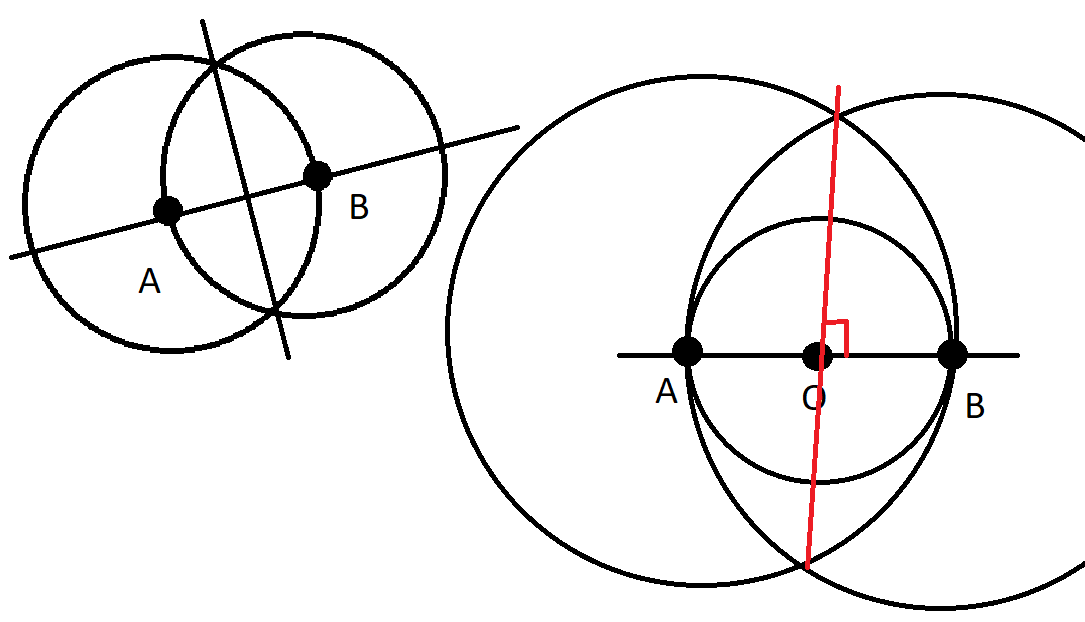
\includegraphics[width=0.7\linewidth]{sections/Ira/images/5-7_2.png}
    \end{minipage}\\
    
    На рисунке слева -- делим отрезок $AB$ пополам (проводя окружности с центром в одной точке и проходящие через другую).
    
    На рисунке справа -- восстанавливаем перпендикуляр из точки $O$. А именно сначала строим произвольную окружность с центром в точке $O$. Отмечаем точки пересечения с прямой $A, B$, а потом отрезок $AB$ <<делим пополам>>.
\end{itemize}
\newpage{}

\section{(10, теорема 1) Теорема о примитивном элементе.}
\Th Пусть $K \supset F$ -- конечное расширение, $char \ F = 0$. Тогда найдется примитивный элемент $\gamma \in K$, т.е. такой, что $K = F(\gamma)$.

\Proof
Так как $K = F(\alpha_1, \ldots, \alpha_n)$, то достаточно доказать утверждение о том, что $F(\alpha, \beta)$ порождается над $F$ одним элементом $\gamma$. Обозначим через $f(x)$ (соотв. $g(x)$) минимальный многочлен над $F$ элемента $\alpha$ (соотв. $\beta$).\\

Идея доказательства в следующем: мы докажем, что $\gamma$ можно взять в виде $\gamma = \alpha + c\beta$ при подходящем
$c \in F$. Окажется, что «плохие» $c$ образуют лишь конечное множество, а значит, ввиду бесконечности $F$ такое $c$ всегда найдётся.\\

Давайте найдем условие на $c$, при котором $F(\alpha, \beta) = F(\gamma)$. Для этого достаточно показать, что $\beta \in F(\gamma)$. Действительно, тогда $\alpha = \gamma - c\beta$ также лежит в $F(\gamma)$, а, значит, $F(\alpha, \beta) \subset F(\gamma)$, и из обратного включения мы получаем требуемое равенство.

Рассмотрим многочлен $h(x) = f(\gamma - cx) \in F(\gamma)[x]$. Элемент $\beta$ является корнем этого многочлена.

Если $deg(h, g) = 1$, то $\beta$ является корнем многочлена первой степени, то есть лежит в $F(\gamma)$.\\

Посмотрим, когда $deg(h, g) > 1$. Так как $g$ не имеет кратных корней, то в $\overline{F}$ найдется корень $\beta_1$ многочлена $g(x)$, отличный от $\beta$, который  является корнем многочлена $h$. Тогда $\alpha_1 = \gamma - c\beta_1$ -- корень многочлена $f(x)$. 

Тогда $\alpha + c\beta = \gamma = \alpha_1 + c\beta_1$, и $c = \frac{\alpha_1 - \alpha}{\beta_1 - \beta}$.

Следовательно, если взять $c \neq \frac{\alpha_1 - \alpha}{\beta_1 - \beta}$ ни для каких сопряженных с $\alpha$ и $\beta$ элементов $\alpha_1$ и $\beta_1$, то $\beta$ будет единственным общим корнем $h, g$, а, значит, $\beta \in F(\gamma)$
\EndProof
\newpage{}

\section{Понятие алгебраической замкнутости и алгебраического замыкания поля. Эквивалентность различных определений (6 штук) алгебраически замкнутого поля}
\Def Поле $K$ называется алгебраически замкнутым, если выполнено одно из следующих эквивалентных условий:

\begin{enumerate}
\item Любой многочлен $f(x) \in K[x]$ с $deg f (x) \geqslant 1$ раскладывается на линейные множители в $K$.
\item  Любой многочлен $f(x) \in K[x]$ с $deg f (x) \geqslant 1$ имеет корень в $K$.
\item Все неприводимые над $K$ многочлены имеют степень 1.
\item Любое алгебраическое расширение над $K$ тривиально (то есть совпадает с $K$).
\item Любое конечное расширение над $K$ тривиально.
\item Для любого многочлена $f(x) \in K[x]$ с $deg f (x) \geqslant 1$ его поле разложения совпадает с $K$.
\end{enumerate}

\Def Алгебраическим замыканием поля $F$ называется алгебраическое расширение $K = \overline{F}$ поля $F$, которое является алгебраически замкнутым полем.

\Proof 
$(1) \Rightarrow (2)$: Тривиально, если многочлен $f: deg f(x) \geqslant 1$ раскладывается на линейные сомножители, то он имеет корень.

$(2) \Rightarrow (3)$: Если многочлен $f$ имеет корень $\alpha \in K$, то $x - \alpha | f$. Тогда, в силу неприводимости, $f \simeq x - \alpha$.

$(3) \Rightarrow (4)$: Пусть $L \supset K$ — алгебраическое расширение, $\alpha \in L$. Рассмотрим минимальный многочлен $m_{\alpha} \in K[x]$ элемента $\alpha$ над $K$. Поскольку $m_{\alpha}$ неприводим, то $deg m_{\alpha} = 1$, откуда $\alpha \in K$.

$(4) \Rightarrow (5)$: Тривиально, поскольку любое конечное расширение является алгебраическим.

$(5) \Rightarrow (6)$: Поле разложения многочлена $f$ является конечным расширением поля $K$, а значит, совпадает с $K$.

$(6) \Rightarrow (1)$: Поле разложения многочлена $f$ совпадает с $K$, значит, $f$ раскладывается на линейные сомножители над $K[x]$.
\EndProof
\newpage{}

\section{Описание группы Галуа $Aut(K)$ поля $K$ разложения многочлена а) $x^4 − 2$; б) $x^4 + 2$ (и похожих). Соответствие подполя $K$ — подгруппы $Aut(K)$ с уточнением о нормальности.}
\par Рассмотрим пункт а) (пункт б аналогично)
\par Поле разложения: $\Q(\sqrt[4]{2}, i)$. Степень разложения 8, значит всего 8 автоморфизмов. Каждый автоморфизм задается тем, куда переходят $\sqrt[4]{2}$ и $i$ (каждый из них пеерходит в какой-то другой корень их минимального могочлена. Получаем
\begin{center}
    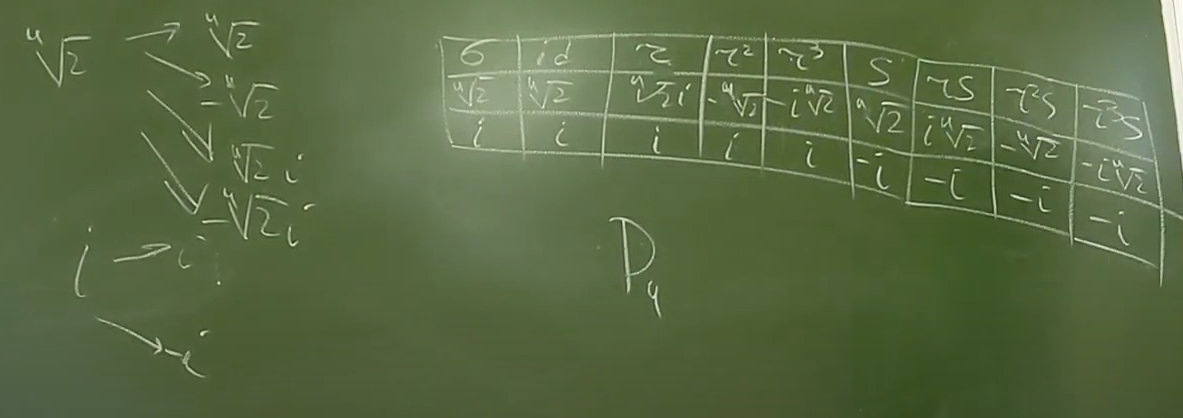
\includegraphics[scale=0.7]{images/automorphisms.png}
\end{center}

\par Что означает табличка: куда переходит $\sqrt[4]{2}$ и $i$. Сначала нашли $r$, посмотрели все комбинации с ним, потом $s$ и посмотрели все комбинации с ним и $r$. Из таблички видим, что структура группы такая же как у $D_4$

\par Для $D_4$ есть нормальная подгруппа порядка 2 из тождественной и центральной симметрии + одна подгруппа порядка 2 $\{id, r^2s\}$. Есть одна подгруппа порядка 4 из поворотов.

\par Остается теперь посмотреть на соответствие полей и подгрупп (TODO чуть поже попробую сделать картинку как на лекции)
\newpage{}

\section{Эквивалентность определений нормального расширения (расширения Галуа).}
\begin{theorem}
	Пусть расширение $L \supset F$ сепарабельно. Тогда следующие условия эквивалентны:
	\begin{enumerate}
		\item Расширение $L$ нормально
		\item $L$ является полем разложения некоторого многочлена $f \in F[x]$
		\item $|Aut_F{L}| = [L : F]$
		\item $L^{Aut_F{L}} = F$
	\end{enumerate}
\end{theorem}

\begin{proof}~
	\begin{itemize}
		\item[$1 \Rightarrow 2$] Рассмотрим $\gamma \in L$ такой, что $L = F(\gamma)$. Все сопряженные с $\gamma$ элементы лежат в $L$, поэтому минимальный многочлен $m_\gamma \in F[x]$ раскладывается на линейные сомножители над $L$. Поскольку $L = F(\gamma)$, то это минимальное поле, удовлетворяющее этому условию. Значит, $L$ "--- это поле разложения многочлена $m_\gamma$.
		\item[$2 \Rightarrow 1$]Пусть $L$ "--- поле разложения многочлена $f \in F[x]$. Рассмотрим произвольный элемент $\gamma \in L$ с минимальным многочленом $m_\gamma \in F[x]$. Пусть $\delta \in L$ "--- сопряженный с ним элемент. Тогда $F(\gamma) \cong F[x]/(m_\gamma) \cong F(\delta)$, причем изоморфизм $\varphi: F(\gamma) \to F(\delta)$ сохраняет $F$. Пока оставим без доказательства, что тогда $\varphi$ можно продолжить до гомоморфизма $\widetilde{\varphi}: L \to \overline{F}$. Но тогда $\widetilde{\varphi}$ переводит корни многочлена $f$ в сопряженные с ними элементы, поэтому $\widetilde{\varphi}(L) \subset L$ и $\delta = \varphi(\gamma) = \widetilde{\varphi}(\gamma) \in L$.
		\item[$1 \Rightarrow 3$] Мы знаем, что $|Aut_{F}L| = |\{\alpha \in L : \alpha\text{ сопряжен с }\gamma\}|$. Тогда, поскольку расширение $L$ нормально, $|Aut_{F}{L}| = [L : F]$.
		\item[$3 \Rightarrow 4$] Пусть $L^{Aut_FL} = K \supset F$, тогда $Aut_FL = Aut_KL$. Мы уже знаем, что всегда выполнено $|Aut_KL| \le [L : K]$. Но тогда $[L : K] \ge |Aut_KL| = |Aut_FL| = [L : F]$, поэтому $[L : K] = [L : F]$ и $K = F$.
		\item[$4 \Rightarrow 1$] Зафиксируем произвольный элемент $\gamma \in L$. Рассмотрим следующий многочлен: $f(x) := \prod_{g \in Aut_FL}(x - g(\gamma)) \in L[x]$. Для любого автоморфизма $h \in Aut_FL$ выполнено $h(f)(x) = \prod_{g \in Aut_FL}(x - h(g(\gamma))) = \prod_{\widetilde{g} \in Aut_FL}(x - \widetilde{g}(\gamma)) = f(x)$. Значит, все коэффициенты многочлена $f$ лежат в $L^{Aut_FL} = F$. Тогда, по построению, любой сопряженный с $\gamma$ элемент является корнем $f$, поэтому он имеет вид $g(\gamma)$ для некоторого $g \in Aut_FL$ и лежит в $L$.\qedhere
	\end{itemize}
\end{proof}

\begin{definition}
	Конечное нормальное сепарабельное расширение $L \supset F$ поля $F$ называется \textit{расширением Галуа}.
\end{definition}

\begin{lemmanote}
	Аналогично доказанному выше, для необязательно сепарабельного расширения $L \supset F$ эквиваленты следующие условия:
	\begin{enumerate}
		\item Расширение $L$ нормально
		\item $L$ является полем разложения некоторого многочлена $f \in F[x]$
		\item Любой гомоморфизм полей $\varphi: L \to \overline{F}$, сохраняющий $F$, является автоморфизмом поля $L$
	\end{enumerate}
	
	Приведем доказательство эквивалентности:
	\begin{itemize}
		\item[$1 \Rightarrow 2$] Пусть элементы $\gamma_1, \dots, \gamma_n \in L$ образуют базис в $L$ над $F$. Рассмотрим их минимальные многочлены $m_{\gamma_1}, \dotsc, m_{\gamma_n} \in F[x]$, тогда, в силу нормальности, все корни этих многочленов лежат в $L$, причем $L$ "--- минимальное по включению поле, содержащее их. Значит, $L$ "--- поле разложения многочлена $m_{\gamma_1}\dotsm m_{\gamma_n}$.
		
		\item[$2 \Rightarrow 3$] Пусть гомоморфизм $\varphi: L \to \overline{F}$ сохраняет $F$. Тогда $\varphi$ осуществляет перестановку корней многочлена $f$, полем разложения которого является $L$, поэтому $\varphi(L) = L$ и $\varphi$ "--- автоморфизм.
		
		\item[$3 \Rightarrow 1$] Пусть $\gamma \in L$ "--- произвольный элемент, $\widetilde\gamma \in \overline{F}$ "--- сопряженный с $\gamma$ элемент. Тогда существует изоморфизм $\varphi: F(\gamma) \to F(\widetilde\gamma)$, сохраняющий $F$. Такой изоморфизм можно продолжить до гомоморфизма $\widetilde\varphi : L \to \overline{F}$, который является автоморфизмом поля $L$ по условию. Значит, $\widetilde\gamma \in L$.
	\end{itemize}

	Действительно, если $L$ "--- поле разложения многочлена $f \in F[x]$, то вложение $\varphi: L \to \overline{F}$, сохраняющее $F$, осуществляет перестановку корней многочлена $f$, поэтому $\varphi(L) = L$ и $\varphi$ является автоморфизмом поля $L$.
\end{lemmanote}
\newpage{}

\section{Основная теорема теории Галуа (формулировка). Доказательство существования биекции между промежуточными полями и подгруппами группы автоморфизмов.}
\par В билетах 12-13 зафиксируем поле $F$ и его расширение Галуа $L \supset F$.
\par \Def Пусть $F$ — поле, $L \supset F$ — его алгебраическое расширение. Элемент $\alpha \in L$ называется сепарабельным, если его минимальный многочлен $m_\alpha$ не имеет кратных
корней над $\overline{F}$. Расширение $L$ называется сепарабельным, если все его элементы сепарабельны.

\par \textbf{Теорема (основная теорема теории Галуа):} Сопоставление $K \mapsto Aut_K L$ (и обратное к нему сопоставление $H \mapsto L^H$) осуществляет биекцию между полями $K$ такими, что
$F \subset K \subset L$ и подгруппами $H \leq Aut_F L$, причем для соответствующих полей $K$ и
подгрупп $H$ выполнено равенство $[Aut_F L : H]=[K:F]$. Более того, расширение $L^H \supset F$ нормально $\Leftrightarrow H \trianglelefteq Aut_F L$.
\par \textbf{Доказательство биективности:} \Proof Проверим, что сопоставления $K \mapsto Aut_K L$ и $H \mapsto L^H$ взаимно обратны:
\begin{itemize}
    \item Пусть $K \mapsto Aut_K L \mapsto L^{Aut_K L}$. Расширение $L \supset K$ нормально в силу нормальности расширения $L \supset F$ (билет 58 на уд), а также сепарабельно и конечно, поэтому $L^{Aut_K L}=K$.
    
    \item Пусть $H \mapsto L^H \mapsto Aut_{L^H} L$. Очевидно, $H \subset Aut_{L^H} L$. Предположим, что $H \subsetneq Aut_{L^H} L$. По теореме о примитивном элементе, $L=L^H(\gamma)$ для некоторого $\gamma \in L$. Рассмотрим многочлен $$f(x):= \prod_{h \in H} (x-h(\gamma)) \in L[x]$$. Поскольку многочлен $f$ сохраняется под действием любого автоморфизма из $H$, то все его коэффициенты лежат в $L^H$. Но $f(\gamma)=0$, поэтому минимальный многочлен $m_\gamma \in L^H[x]$ делит $f$. Тогда, поскольку $L \supset L^H$ является расширением Галуа, выполнено $\deg m_\gamma \leq \deg f = |H| < |Aut_{L^H} L|=[L:L^H]=\deg m_\gamma$ — противоречие. 
\end{itemize}
\par Значит сопоставление является биекцией \EndProof

\section{Основная теорема теории Галуа (формулировка). Уточнение для нормальных подгрупп}
\par \textbf{Доказательство равенства и уточнения:} \Proof Равенство $[Aut_F L : H] = [K : F]$ очевидно,
поскольку $|Aut_K L|=[L:K]$ и $|Aut_F L| =[L:F]$. 

\par Наконец, заметим, что $\forall g \in Aut_F L$
выполнено $L^{gHg^{-1}}=\{x \in L: \forall h \in H: h(g^{-1}(x))=g^{-1}(x)\}=\{g(x): x\in L^H\} = g(L^H)$. Значит, $H \trianglelefteq Aut_F L \Leftrightarrow \forall g \in Aut_F L: g(L^H)=L^H \Leftrightarrow$ расширение $L^H \supset F$ нормально. Последний переход слева направо выполнен потому, что изоморфизм $\varphi: F(\alpha)\rightarrow F(\tilde{\alpha})$,
сохраняющий $F$ и переводящий $\alpha \in L^H$ в сопряженный с ним элемент $\tilde{\alpha}$, можно продолжить до некоторого гомоморфизма $\tilde{\varphi}:L \rightarrow \overline{F}$, причем, в силу нормальности расширения $L \supset F$, $\tilde{\varphi}$ является автоморфизмом поля $L$ \EndProof

\newpage{}

\section{Теорема о построимости комплексного числа при помощи циркуля и линейки через поле разложение многочлена (в одну сторону).}
\par \Statement Пусть $G$ — конечная группа порядка $2^n, n \in \N$. Тогда в $G$ есть подгруппа $H$ такая, что $[G:H]=2$.
\par \Proof Проведем индукцию по $n$. База, $n=1$, тривиальна, докажем переход.
\par Группа $G$ является $p$-группой, поэтому ее центр $Z(G)$ нетривиален. Поскольку $Z(G) \trianglelefteq G$,
можно рассмотреть группу $G/Z(G)$. Это 2-группа меньшего порядка, и по предположению индукции в $G/Z(G)$ есть подгруппа $H$ такая, что $[G/Z(G) : H]=2$. По теореме о
соответствии, $H=K/Z(G)$ для некоторой группы $K$ такой, что $Z(G) \leq K \leq G$. Значит, $[G:K]=2$, и переход доказан.

\par \Cor Пусть $G$ — группа, $|G|=2^n$. Тогда в $G$ существует такая цепочка подгрупп $G=G_n \geq G_{n-1} \geq \ldots \geq G_0 = \{e\}$, что $\forall i \in \{0, \ldots, n-1\}: [G_{i+1}:G_i]=2$.

\par \Th Точку $z \in \Comp$ можно построить циркулем и линейкой $\Leftrightarrow$ поле разложения ее минимального многочлена $m_z \in \Q[x]$ имеет степень $2^n, n \in \N$.
\par \textbf{Доказательство достаточности (справа налево):} \Proof Обозначим через $L$ поле разложения многочлена $m_z$.
Пусть $[L : \Q]=2^n, n \in \N$. Тогда в группе $G:=Aut_\Q L$ порядка $2^n$ существует такая цепочка подгрупп $G=G_n \geq \ldots \geq G_0=\{e\}$, что для всех $i \in \{0, \ldots, n-1\}$ выполнено $[G_{i+1} : G_i]=2$. Выберем соответствующую цепочке подгрупп башню расширений $\Q=L_n \subset \ldots \subset L_0=L$, тогда $\forall i \in \{0, \ldots, n-1\}: [L_i : L_{i+1}]=2$. Но $x \in L$, поэтому $x$ можно построить по уже доказанному критерию (см. билет 7 на отл). \EndProof
\par TODO возможно нужно доказательство в другую сторону?
\newpage{}

\section{Теорема о минимальном многочлене примитивного корня $n$-ой степени из 1. Построимость правильного $n$-угольника при помощи циркуля и линейки (док-во через теорию Галуа)}
\par \Th Степень минимального многочлена числа $\xi_n \in \Comp$ над $\Q$ равна $\varphi(n)$.

\par \Proof Для произвольного $n \in \N$ положим 

$$\psi_n(x):=\prod_{\substack{1\leq d \leq n, \\ (d,n)=1}} (x-\xi_n^d)$$

\par Докажем, что это минимальный многочлен для $\xi_n$ над $\Q$. Проверим сначала, что $\psi_n \in \Z[x]$.
Действительно, поскольку выполнено равенство $\prod_{k|n} \psi_k(x)=x^n-1$ (???), то целочисленность всех коэффициентов многочлена $\psi_n$ легко проверяется по индукции.

\par Пусть теперь $m \in \Q[x]$ — минимальный многочлен для $\xi_n$ (возможно, отличный от $\psi_n$), $\xi$ — его произвольный корень. Покажем, что $m$ должен также иметь корни $\xi^p$ для всех
простых чисел $p \nmid n$. В силу минимальности, $m | x^n-1$, то есть $x^n-1=m(x)g(x)$ для некоторого $g \in \Q[x]$, причем коэффициенты многочленов $m,g$ целочисленны, поскольку многочлен $x^n-1$ примитивен и имеет старший коэффициент, равный 1. 

\par Предположим, что $m(\xi_p)\neq 0$, тогда $g(\xi_p)=0$, поэтому $m | g(x^p)$, то есть выполнено равенство $g(x^p)=m(x)h(x)$ для некоторого $h \in \Q[x]$, и, аналогично, коэффициенты многочлена $h$ целочисленны. В поле $\Z_p$ равенство принимает вид $\overline{g}(x^p)=\overline{g}(x)^p=\overline{m}(x)\overline{h}(x)$. Значит, в алгебраическом замыкании поля $\Z_p$ многочлены $\overline{g}$ и $\overline{m}$ имеют общий корень. Но многочлен $x^n-1$ не имеет кратных корней, поскольку его формальная производная равна $nx^{n-1}$ и не имеет корней, отличных от нуля. Значит, $m(\xi^p)=0$. Но тогда и для всех чисел $d \in \N$ таких, что $(d,n)=1$, выполнено $m(\xi_n^d)=0$. Значит, минимальный многочлен $m$ совпадает с $\psi_n$ и имеет степень, равную $\varphi(n)$. \EndProof

\par \Cor Пусть $n \in \N$. Тогда правильный $n$-угольник можно построить циркулем и линейкой $\Leftrightarrow \varphi(n)=2^k, k\in \N$
\par \Proof Очевидное следствие из этой теоремы и теоремы из билета 14 на отл \EndProof
\newpage{}

\section{Aвтоморфизм Фробениуса. Группа Галуа конечного расширения.
Равенство $\deg \Psi_{n, Z_p} = ord_n(p)$.}
\par Пусть $F \supset \Z_p$, $|F|=p^n$
\par \Def $\sigma(a)=a^p$ - автоморфизм Фробениуса
\par То что это автоморфизм очевидно, так как
$$(a+b)^p=a^p+b^p, \quad (ab)^p=a^pb^p$$
\par Посмотрим какие элементы сохраняет $\sigma$: $a^p=\sigma(a)=a \Rightarrow a$ - корень многочлена $x^p-x \Rightarrow a \in \Z_p$. То есть $\sigma$ сохраняет $\Z_p$.
\par Другие автоморфизмы: $\sigma^k: \: a \mapsto a^{p^k}$. Помним, что $F$ - поле разложения многочлена $x^{p^n}-x$. Допустим у нас так не наберется $n$ автоморфизмов. Тогда $\exists k < n: \forall a \in F \: a^{p^k}=\sigma^k(a)=a \Rightarrow \forall a \in F$ - корень $x^{p^k}-x \Rightarrow$ всего таких $a$ не больше $p^k<p^n$ - противоречие.

\par $F \supset \Z_p$ - нормальное (так как это поле разложения), значит $|Aut_{\Z_p} F|=n \Rightarrow Aut_{\Z_p} F=\langle \sigma \rangle$.

\par \Statement $K \supset L$ - расширение, $|K|=p^n, |L|=p^k$ и $n \: \vdots \: k$. Тогда $Aut_L K=\langle \tau \rangle$, $\tau(a)=a^{p^k}$
\par \Proof Действуем аналогично тому что расписали выше. $K \supset L \supset \Z_p$
\begin{enumerate}
    \item $\tau$ сохраняет $L$, так как $L$ - поле разложения $x^{p^k}-x$
    
    \item $\tau, \tau^2, \ldots, \tau^l=id$
    \par $\tau^l(a)=a^{p^{kl}} \Rightarrow l = \frac{n}{k}$
    
    \item $|Aut_L K|=[K:L]=\frac{n}{k}=l \Rightarrow Aut_L K=\langle \tau \rangle$ \EndProof
\end{enumerate}
\par \textbf{Вывод:} в поле из $p^n$ элементов $\exists !$ подполе из $p^k$ элементов, где $n \: \vdots \: k$.

\par \Def $\Psi_{n, F}(x)=m_{\xi_n,F}(x)$ - многочлен деления круга

\par \Statement $\deg \Psi_{n, \Z_p}(x)=ord_n(p)$
\par \Proof $\xi:=\xi_n$ - корень $\Psi_{n, \Z_p}(x), \deg \Psi_{n, \Z_p}(x)=k$. $\xi^n=1, \xi^k \neq 1$ при $k < n$.
\par Пусть $F=\Z_p(\xi), |F|=p^k$. Рассмотрим $\xi, \xi^p, \xi^{p^2}, \ldots, \xi^{p^k}=\xi$ - сопряженные элементы к $\xi$ над $\Z_p$. Следовательно, $\xi^{p^k-1}=1 \Rightarrow p^k-1 \: \vdots \: n \Rightarrow p^k \equiv 1 (n)$.

\par Если $p^l \equiv 1(n) \Rightarrow \xi^{p^l-1}=1 \Rightarrow \xi^{p^l}=\xi \Rightarrow l \geq k$ (так как при $l<k$ элементы сопряжены с $\xi$, но не совпадают) $\Rightarrow k = ord_n(p)$ \EndProof
\newpage{}

\section{Основная теорема алгебры (доказательство через теорию Галуа).}
\par \textbf{Теорема (основная теорема алгебры):} Поле $\Comp$ алгебраически замкнуто.
\par \Proof Заметим, что верны два следующих утверждения:
\begin{enumerate}
	\item Каждый многочлен $f \in \R[x]$ нечетной степени имеет корень.
	\item Каждый многочлен $g \in \Comp[x]$ степени $2$ имеет корень.
\end{enumerate}

\par Из этого следует, что у $\R$ нет нетривиальных конечных расширений нечетной степени, а у $\Comp$ нет конечных расширений степени $2$. Действительно, по теореме о примитивном элементе, такое расширение порождалось бы одним элементом, и его минимальный многочлен был бы неприводим и при этом имел бы корень.

\par Пусть $L \supset \Comp$ "--- конечное расширение. Тогда расширение $L \supset \R$ тоже конечно, поэтому $L = \R(\gamma)$ для некоторого $\gamma \in L$. Рассмотрим $K \supset L$ "--- поле разложения минимального многочлена $m_\gamma \in \R[x]$, тогда расширения $K \supset\R$ и $K \supset \Comp$ нормальны. Выберем силовскую $2$-подгруппу $H$ в $Aut_{\R}K$ и соответствующее ей поле $M$ такое, что $\R \subset M \subset K$. Тогда $[M : \R] = [Aut_{\R}K : H] \equiv_2 1$, поэтому $M = \R$. Значит, $[K : \R] = [K : M] = |H| = 2^n$, $n \in \N$. Тогда $[K : \Comp] = 2^{n - 1}$. Если $n \ge 2$, то, аналогично, выберем подгруппу индекса $2$ в $Aut_{\Comp}K$ и получим расширение поля $\Comp$ порядка $2$, что невозможно. Значит, $n = 1$ и $K = L = \Comp$.

\par Таким образом, у поля $\Comp$ нет нетривиальных конечных расширений, поэтому оно алгебраически замкнуто. \EndProof
\newpage{}

\section{Теорема о примитивном элементе для конечных полей.}
\par \textbf{Теорема (о примитивном элементе):} Пусть $F$ — конечное поле, $K \supset F$ — конечное расширение поля $F$. Тогда существует $\gamma \in K$ такой, что $K=F(\alpha)$.
\par \Proof $K^*$ - циклическая группа. Пусть $K=\langle a \rangle$.
\par Так как $K=K^* \cup \{0\}$, то $K=F(a)$ значит примитивный элемент найден \EndProof
\newpage{}

\section{Группа Галуа расширений $x^n − 1$ и $x^n − a$ (второе над полем, содержащим все корни $n$-й степени из 1).}
\par \Def Расширение Галуа $K \supset F$ называется циклическим (абелевым), если $Aut_F K$ - циклическая (абелева)

\par \Statement $K \supset F$ - поле разложение $x^n-a \Rightarrow K \supset F$ - абелево

\par \Proof Будем строить расширение $K$ в два этапа $K \supset L \supset F$, где $L$ - поле разложения $x^n-1$
\begin{enumerate}
    \item $L=F(\xi_n)$, где $\xi_n$ - корень $n$-ой степени из 1. Пусть $\varphi \in Aut_F L$. Тогда $\varphi(\xi_n)=\xi_n^l, l \in \Z_n^*$ (так как $F$ переходит в себя под действием $\varphi$). Значит каждое отображение из $Aut_F L$ однозначно задается степенью $l$, в которую переходит корень из 1 (обозначим соответствующий автоморфизм как $\varphi_l$). Рассмотрим композицию
    $$\varphi_l \circ \varphi_k(\xi_n) = \varphi_l(\varphi_k(\xi_n))=\varphi_l(\xi_n^k)=(\varphi(\xi_n))^k=\xi^{kl}$$
    \par Получаем, что $Aut_F L \subset \Z_n^*$ (отображение $\varphi_l \mapsto l$), а значит $Aut_F L$ - абелева (но необязательно циклическая)
    
    \item Корни $x^n-a$: $\sqrt[n]{a}, \sqrt[n]{a}\xi_n, \ldots, \sqrt[n]{a}\xi_n^{n-1}$. Поэтому $K=L(\sqrt[n]{a})$.
    \par Рассмотрим $\psi \in Aut_L K$. $\psi_k(\sqrt[n]{a})=\sqrt[n]{a} \xi_n^k$ (по соображением аналогичным пункту 1). Опять занумеруем $\psi$ и рассмотрим композицию, помня, что все $\psi$ оставляют $L$ на месте
    $$\psi_l \circ \psi_k(\sqrt[n]{a})=\psi_l(\sqrt[n]{a} \xi_n^k)=\psi_l(\sqrt[n]{a})\psi_l(\xi_n^k)=\sqrt[n]{a}\xi_n^k \xi_n^l=\psi_{l+k}(\sqrt[n]{a})$$
    \par Отсюда следует, что $Aut_L K \cong \Z_n$ ($\Z_n$ - группа по сложению), а значит $Aut_L K$ - абелева (и циклическая).
\end{enumerate}
\par Таким образом, получаем, что $K$ - абелево \EndProof
\newpage{}

\section{Разрешимость в радикалах. Три формулировки, эквивалентность первых двух.}
\Def Уравнение $f(x) = 0$ \textbf{разрешимо в радикалах} над $\Q$, если выполнено одно из следующих условий:

\begin{enumerate}
\item $\exists$ $\alpha$ - корень многочлена $f(x)$: $\alpha \in K = K_0 \supset K_1 \supset \dots \supset K_n = \Q$; $K_i = K_{i+1}(a_i), a_i^{m_i} \in K_{i+1}$ 
\item $\forall$ $\alpha$ - корень многочлена $f(x)$: $\alpha \in K = K_0 \supset K_1 \supset \dots \supset K_n = \Q$; $K_i = K_{i+1}(a_i), a_i^{m_i} \in K_{i+1}$

\end{enumerate}

\Note Вместо $\Q$ может быть любое другое поле.

\Note Идейно мы хотим сказать, что разрешимо в радикалах - значит, можно получить ответ при помощи операция $+, -, \cdot, \backslash$ и $\sqrt[n]{}$

\Note Из 1 следует 2 (и наоборот, очев), но док-во технически сложное и не приводится. 

\Note Проблемы с определением 1: хотим, чтобы $K$ было нормальным над $\Q$; так же хочется, чтобы K было похоже на поле разложения многочлена.

Отсюда 3 определение: $K_i$ - поле разложения $x^{m_i} - a_i$ над $K_{i+1}$.

Не решает первую проблему, т.к. \Example 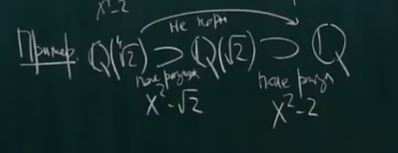
\includegraphics[]{images/5_19.JPG}

\textbf{Идея:} также брать $x^{m_i} - \overline{a_i}$ для всех сопряжённых к $a_i$.

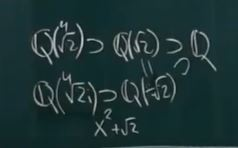
\includegraphics[]{images/5_19_2.JPG}

\Th $f(x) = 0$ разрешимо в радикалах $\Leftrightarrow$ Существует башня расширений $L = L_0 \supset L_1 \supset \dots \supset L_n = \Q$ такая, что для каждого $i \in \{0, 1, \dots, n-1 \}$ поле $L_i$ — это поле разложения многочлена $x^{m_{i+1}} - a_{i+1} \in L_{i+1}[x]$ (одно из определений разрешимости в радикалах)

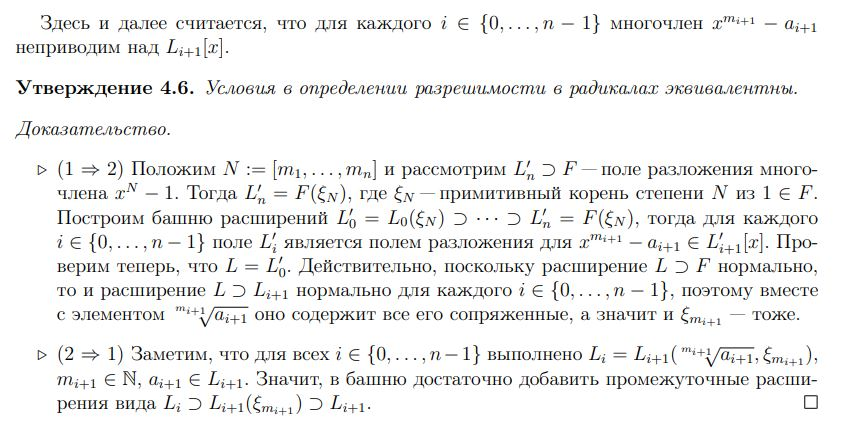
\includegraphics[]{images/5_19_3.JPG}

\section{Разрешимость в радикалах. Сведение к вопросу о разрешимости группы Галуа. Формулировка основной теоремы, доказательство в одну сторону}
\Def  Группой Галуа многочлена $f \in F[x]$ называется группа автоморфизмов, сохраняющих $F$, его поля разложения. Обозначение — $Gal f$

\Def Группа $G$ разрешимая, если $\exists n \in \N $: n-ый коммутант $G^{(n)}$ тривиален.

\Note Из теории групп: разрешимость $\Leftrightarrow $ в G $\exists$ цепочка $G = G_n \unrhd G_{n-1} \dots \unrhd G_{0} = e$: $\forall i$ фактор-группа $G_{i+1}\backslash G_i$ абелева.

\Th Для $f(x) \in F[x]$ $f(x) = 0$ разрешимо в радикалах $\Leftrightarrow$ Gal $f$ разрешима.

\Proof 
Пусть $L = L_0 \supset \dotsb \supset L_n = F$ "--- башня расширений из определения разрешимости в радикалах. Проверим, что $\Gal{f} = \Aut_{L_n}{L} \ge \dotsb \ge \Aut_{L_0}L = \{\id\}$ при добавлении нескольких промежуточных подгрупп образует цепочку нормальных подгрупп с абелевыми факторами.
		
		Для произвольного $i \in \{0, \dotsc, n - 1\}$ рассмотрим многочлен $x^{m_{i+1}} - a_{i+1} \in L_{i + 1}[x]$, полем разложения которого является $L_i$, а также $K_i$ "--- поле разложения многочлена $x^{m_{i+1}} - 1 \in L_{i + 1}[x]$, тогда $L_i = L_{i + 1}(\sqrt[\leftroot{2}\uproot{4}m_{i+1}]{a_{i+1}}, \xi_{m_{i+1}}) \supset K_i = L_{i + 1}(\xi_{m_{i+1}}) \supset L_{i + 1}$.
		
		Каждый автоморфизм $\phi \in \Aut_{L_{i+1}}K_i$ однозначно задается образом элемента $\xi_{m_{i+1}}$, а $\xi_{m_{i+1}}$ может переходить только в один из элементов вида $\xi_{m_{i+1}}^m$, где $m \in \N$ "--- такое, что $(m, {m_{i+1}}) = 1$, причем композиция автоморфизмов соответствует умножению степеней элемента $\xi_{m_{i+1}}$. Значит, $\Aut_{L_{i+1}}K_i \subset \Z_{m_{i+1}}^*$, поэтому группа $\Aut_{L_{i+1}}K_i$ "--- абелева.
		
		Аналогично, каждый автоморфизм $\phi \in \Aut_{K_i}L_i$ однозначно задается образом элемента $\sqrt[\leftroot{2}\uproot{4}m_{i+1}]{a_{i+1}}$, а $\sqrt[\leftroot{2}\uproot{4}m_{i+1}]{a_{i+1}}$ может переходить только в один из элементов вида $\sqrt[\leftroot{2}\uproot{4}m_{i+1}]{a_{i+1}}\xi_{m_{i+1}}^m$, где $m \in \{0, \dotsc, m_{i+1} - 1\}$, причем композиция автоморфизмов соответствует сложению степеней элемента $\xi_{m_{i+1}}$. Значит, $\Aut_{K_i}L_i \subset \Z_n$, поэтому группа $\Aut_{K_i}L_i$ "--- тоже абелева.
		
		Заметим теперь, что $\Aut_{K_i}L \normal \Aut_{L_{i + 1}}L$ и $\Aut_{L_{i}}L \normal \Aut_{K_i}L$, поскольку расширения $K_i \supset L_{i+1}$ и $L_i \supset K_i$ нормальны. Применим теорему о гомоморфизме к сопоставлениям $\phi \mapsto \phi|_{K_i}$ и $\psi \mapsto \psi|_{L_i}$, где $\phi \in \Aut_{L_{i + 1}}L$, $\psi \in \Aut_{K_i}L$, и получим, что $\Aut_{L_{i+1}}K_i \hm\cong \Aut_{L_{i + 1}}L / \Aut_{K_i}L$ и $\Aut_{K_i}L_i \cong \Aut_{K_i}L / \Aut_{L_i}L$. Следовательно, $\Gal{f} = \Aut_{L_n}{L} \varnormal \Aut_{K_{n-1}}L \varnormal \dotsb \varnormal \Aut_{K_0}L \varnormal \Aut_{L_0}L = \{\id\}$ "--- это цепочка нормальных подгрупп с абелевыми факторами.
		
\EndProof
\newpage{}

\section{Разрешимость в радикалах. Пример уравнения, неразрешимого в радикалах над Q.}
\Cor
	Пусть $f \in \Q[x]$ "--- неприводимый многочлен степени $5$, имеющий над $\R$ ровно $3$ корня. Тогда уравнение $f(x) = 0$ не разрешимо в радикалах.

\Proof
	Можно считать, что каждый автоморфизм из $\Gal{f}$ осуществляет перестановку корней многочлена $f$ над $\overline{\Q}$, поэтому $\Gal{f} \subset S_5$. Пусть корни $\alpha_1, \alpha_2 \in \overline{\Q}$ многочлена $f$ "--- комплексные, а остальные "--- вещественные. Тогда комплексное сопряжение, то есть $(12) \in S_5$, лежит в $\Gal{f}$. В силу утверждения о продолжении гомоморфизма, для любых $i, j \in \{1, \dotsc, 5\}$ существует автоморфизм из $\Gal{f}$ такой, что $\alpha_i \mapsto \alpha_j$. Докажем теперь, что из этого следует равенство $\Gal{f} = S_5$.
	
	Рассмотрим граф транспозиций в $\Gal{f}$, то есть граф с множеством вершин $\{1, \dotsc, 5\}$ и множеством ребер $\{\{i, j\} : (ij) \in \Gal{f}\}$. Поскольку $\Gal{f}$ "--- группа, то компоненты связности в этом графе являются кликами. Заметим теперь, что при сопряжении перестановкой $\sigma \in \Gal{f}$ такой, что $\sigma(i) = j$, компонента, содержащая $i$, переходит в компоненту, содержащую $j$. Значит, все компоненты имеют одинаковый размер. Но число $5$ "--- простое, поэтому в графе есть лишь одна компонента, и, следовательно, $\Gal{f} = S_5$. Эта группа неразрешима, поэтому и уравнение $f(x) = 0$ не разрешимо в радикалах.
\EndProof

\Example
	Многочлен $f := x^5 - 10x + 5 \in \Q[x]$ не разрешим в радикалах. Действительно, исследуя $f$ на экстремумы, легко проверить, что он имеет ровно три корня над $\R$, а его неприводимость следует из признака Эйзенштейна по модулю $5$. Значит, применимо утверждение выше.
\newpage{}

\section{Теория Кумера. Теорема Артина о характерах.}
\Th \textbf{Теория Кумера}: $K \supset F$ - расширение Галуа, причём в $F$ лежат все корни n-ой степени из 1; $[K : F] = n$. Тогда $K$ циклическое $\Leftrightarrow$ $K$ - поле разложения для какого-то $x^n - a$, $a \in F$

\Proof 
$\Leftarrow$: доказано.

$\Rightarrow$: $Aut_F K = < \sigma > $ - циклическая; $\xi_n$ - примитивный корень n-ой степени из 1. Если всё хорошо, то для искомого $a$ верно $\sigma(a) = \xi_n a, \sigma^k(a) = \xi^k_n a, \sigma^n(a) = a, \sigma(a^n) = a^n$

$(1 + \xi_n \sigma + \xi_n^2 \sigma^2 + \dots + \xi_n^{n-1} \sigma^{n-1})(\beta) = \theta$

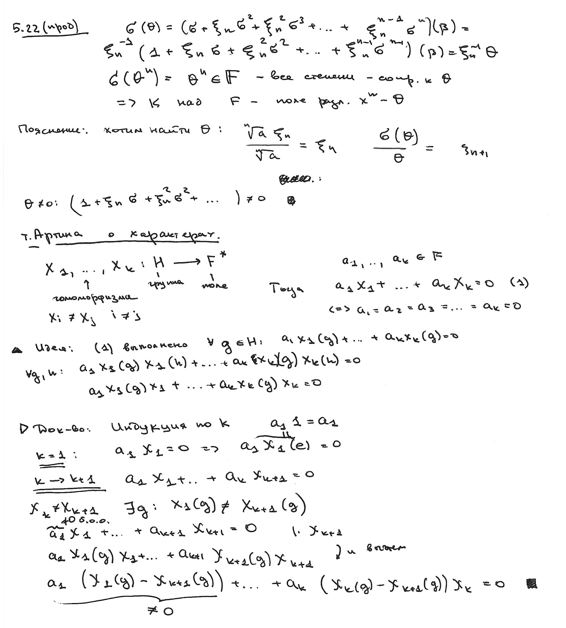
\includegraphics[]{images/5_22.JPG}
\newpage{}

\section{Группы Галуа для неприводимых многочленов 3-й и 4-й степени.}
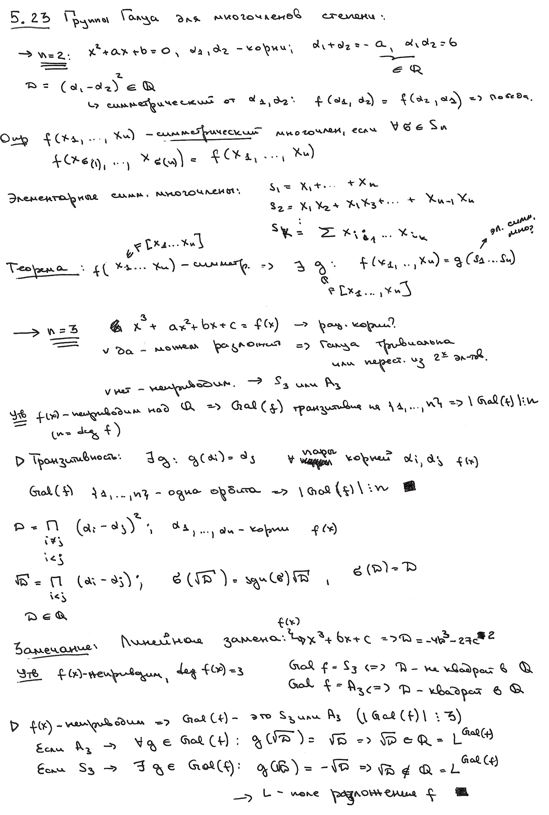
\includegraphics[]{images/5_23_1.JPG}
\\
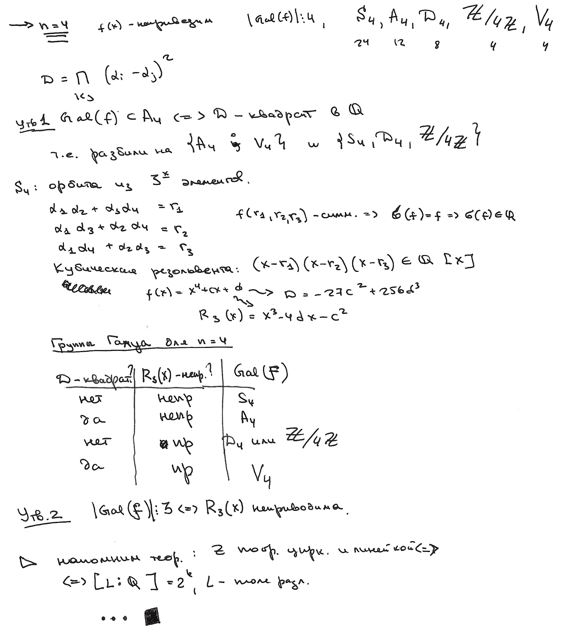
\includegraphics[]{images/5_23_2.JPG}
\newpage{}